 
\section{Paketų atsiskyrimas ir deformacija}
\label{app:negative_current}

\begin{figure}
\subfloat[\(t=0\)ms]{\label{video:1}
\centerline{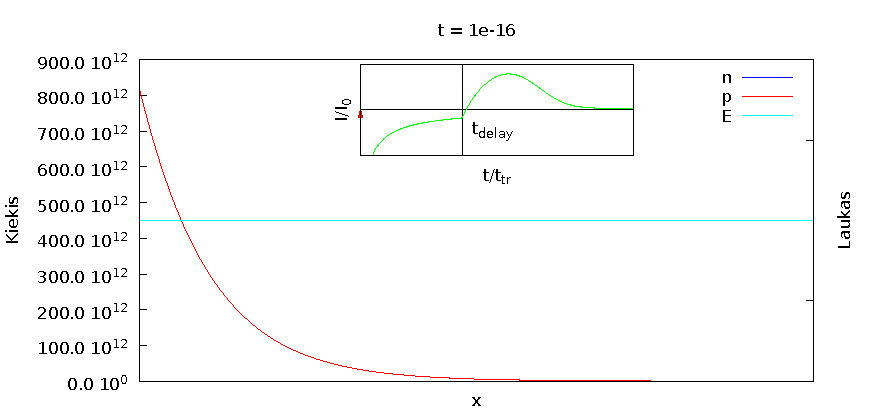
\includegraphics[height=0.28\textheight]{./media/video/00000.pdf}
}}\\
\subfloat[\(t=0.005\)ms]{\label{video:2}
\centerline{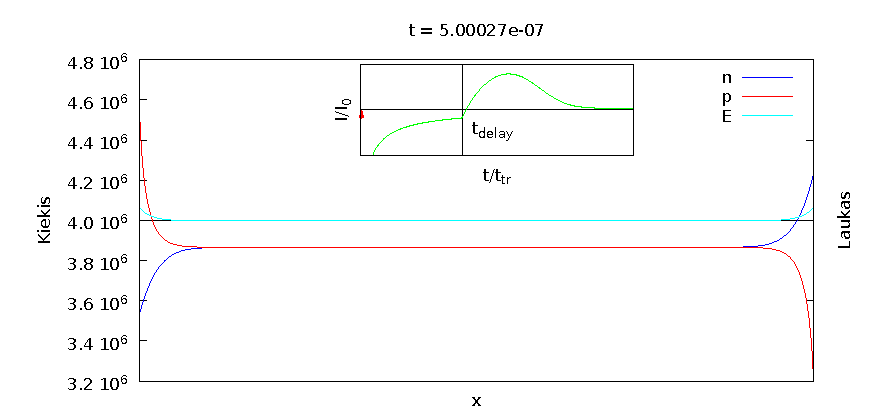
\includegraphics[height=0.28\textheight]{./media/video/00005.pdf}
}}\\
\subfloat[\(t=0.08\)ms]{\label{video:3}
\centerline{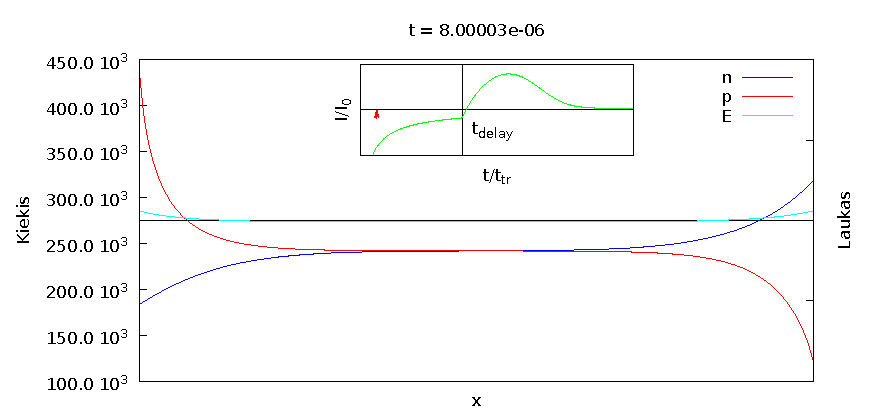
\includegraphics[height=0.28\textheight]{./media/video/00080.pdf}
}}
\caption{Simuliacijos būsenos kitimas laike}
\end{figure}

\begin{figure}
\ContinuedFloat
\subfloat[\(t=0.24\)ms]{\label{video:4}
\centerline{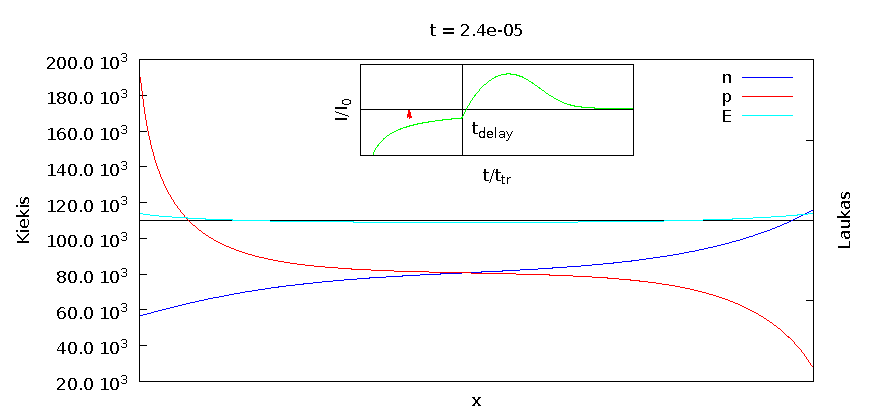
\includegraphics[height=0.28\textheight]{./media/video/00240.pdf}
}}\\
\subfloat[\(t=0.5\)ms]{\label{video:5}
\centerline{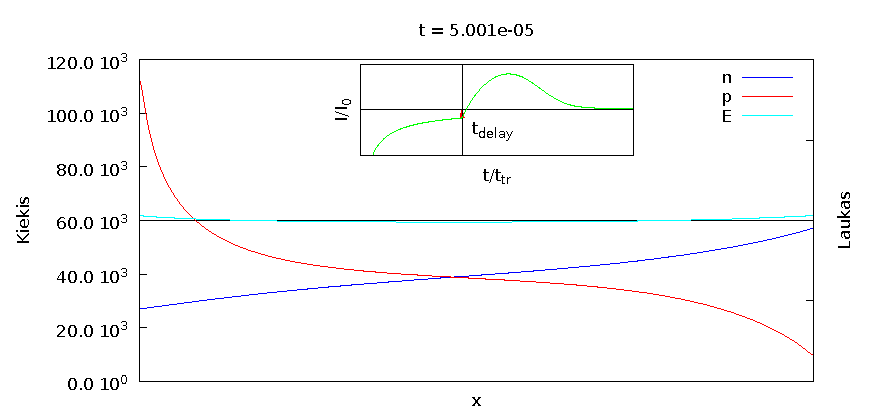
\includegraphics[height=0.28\textheight]{./media/video/00500.pdf}
}}\\
\subfloat[\(t=0.65\)ms]{\label{video:6}
\centerline{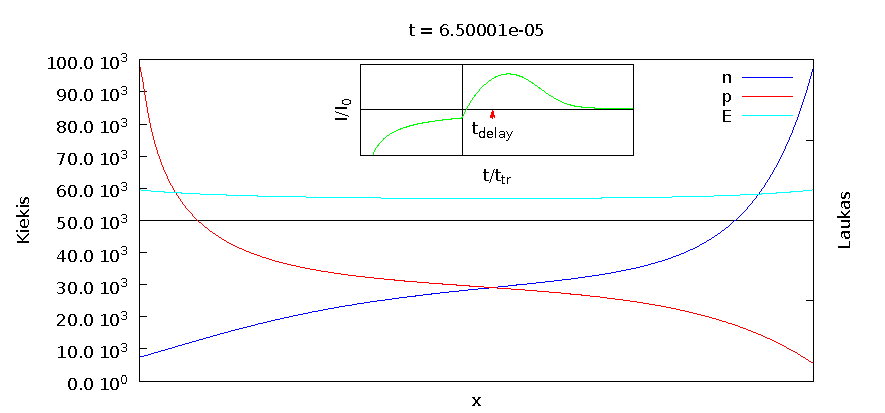
\includegraphics[height=0.28\textheight]{./media/video/00650.pdf}
}}
\caption{Simuliacijos būsenos kitimas laike (tęs.)}
\label{fig:video}
\end{figure}

Pagal darbe aprašytus simuliacijos parametrus (žr. \ref{page:params} skyrelį),kai $\alpha d = 10$, atlikti skaičiavimai, kurių rezultatų pavyzdžiai pateikti \ref{fig:video} pav.
Juose pavaizduoti krūvininkų tankių ir elektrinio lauko pasiskirstymai, skirtingais laiko momentais. Viduryje pavaizduota apskaičiuotoji CELIV kinetika, čia raudona rodyklė žymi laiko momentą, kurio metu sistemos būsena pavaizduota išoriniame paveiksliuke. Nekintanti vertikali juoda linija žymi CELIV signalo pradžią.
Matome, jog pradiniais laiko momentais (\ref{video:1}, \ref{video:2}, \ref{video:3}) krūvininkų tankių pasiskirstymai atsiskiria vienas nuo kito dėl Demberio efekto ir rekombinacijos. Tarp krūvininkų atsiranda nedidelis elektrinis laukas, žymimas žalia linija, čia juoda horizontali juoda linija žymi lauką $E=0$. Dėl elektrinio lauko atsiranda dreifo srovė. Dėl lėtesniųjų krūvininkų nejudrumo rekombinacijos sparta priklauso nuo koordinatės, taigi sukuriamas neigiamas greitesniųjų krūvininkų tankio gradientas kuris kuria difuzijos srovę. Taigi neigiamą srovę kuria difuzinė ir dreifinė komponentės. Vėliau neigiama srovė mažėja, nes krūvininkai artėja link pusiausvyros busenos. Nepasiekus pusiausvyros įjungiamas CELIV signalas ir krūvininkai traukiami prie kontaktų (\ref{video:5}, \ref{video:6}).